\section*{Technical Details of the Optimizer}
\begin{itemize}

\item Experimental Recording Features from Neuroelectro. And some from the Allen SDK.
\item The algorithms IBEA and NSGA2 seem to result in similar optimization convergence speeds, and similar solution quality.

%\item Python, NeuroUnit, 

\subsetion{Model/Test combinations}

Contrast with other optimization approaches:


There are two different strategies, one strategy involves evaluating goodness of fit, only at one current injection strength for every gene. Another approach is a bit more generous, in that, rather than allowing models to instantly fail to evoke a spike at the appropriate current injection, that models specific rheobase value is found, and all other tests are evaluated at the current injection value. The consequence of accomodating poorer fits on the Rheobase test, is allows models to compete on the other seven or more different fitness criteria.

\subsection{Elephant Test Suite}
At a count of eight tests (five useable) the elephant derived suite was relatively compact. The elephant tests suite is concerned with core ephysiology measurements, the particular measurements chosen were important because, for example capacitance, and input resistance directly affect the evolution of reduced model governing equations. Taken as a collection these ephysiological properties as a collection also determine spiking waveform shape. 

Capacitance, Rheobase, Time Constant, Input Resistance, Resting Potential

\item Result It when models were fitted using the following measurements alone, the resulting models were also fitted to spike half-width, arguably because the membrane time-constant, and membrane capacitance together encode spike-half width.

\subsection{Electrophysiology Feature Extraction Library}

Many of the EFEL measurements, and Allen SDK Feature measurements pertain to spike train statistics, because model fitting to spike train statistics is a productive and well understood domain, we did not utilize spike train statistics in model fitting. Instead EFEL spike shape and electrophysiology measurements were applied.\\
\\
Through trial and error experimentation the following EFEL features were demonstrated to result in helpfull and tractible error surfaces. In simulated constraint paradigms using the aforementioned EFEL fitness criteria, lead to recovery of optimal models. This finding did not apply to the entire collection of EFEL features however.\\
\\
In a large scale analysis of variance between models and data see section large_scale_variance

\href{run:./RESULTS_large_scale_variance.tex}{RESULTS_large_scale_variance.tex}

\begin{verbatim}
'AHP_depth_abs_3.0x','sag_ratio2_3.0x','ohmic_input_resistance_1.5x','sag_ratio2_1.5x','peak_voltage_3.0x','peak_voltage_1.5x','voltage_base_3.0x','voltage_base_1.5x','Spikecount_1.5x','Spikecount_3.0x','ohmic_input_resistance_vb_ssse_1.5x'
\end{verbatim}


\item Unlike in BluePyOpt \cite{Werner} and Allen Institute optimization workflows \cite{gouwens} rheobase current injection was applied is a soft constraint. 

However, this work differs from other work in that rheobase current injection was found for every different model paramerisation.\\
\\
\item Rheobase value as a soft constraint. This means that current injection values are a variable model parameter. The exact value of current used is determined via exploring the model response to current injections of varying amplitude. The exact value, its value is determined by other model parameters.

\item spike shape measurements and error functions. We used a set of 8 different experimental measurements NeuronUnit.
\end{itemize}


\begin{figure}
	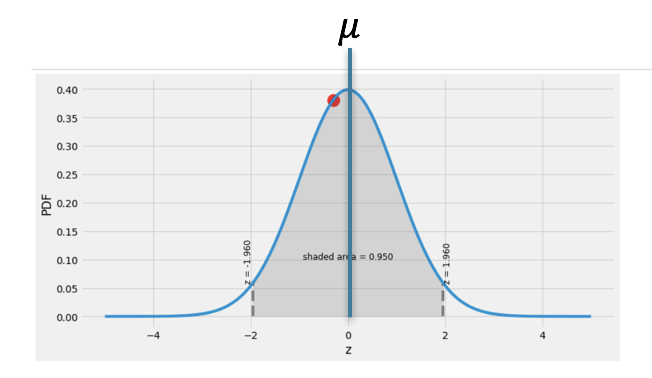
\includegraphics[width=\maxwidth{\textwidth}]{chapters/figures/normal_distribution.png}
    \caption{Error functions were evaluated with the assistance of a library: \emph{NeuronUnit} 
    were based on finding a normal distribution on electro physiology measurements, 
    and then measuring model outputs and mapping the model behavior onto
     a place on the experimental normal distribution. Scores that where closer to the
      experimental mean where deemed to be low in error.
	Z-scores obtained via NeuronUnit can be thought of as  }
	\label{figure\arabic{figurecounter}}
	
\caption{Caption}
	
\end{figure}
